\documentclass[11pt,a4paper]{article}
\author{TalentSprint}
\date{}
\usepackage{graphicx}
\usepackage{verbatim}
\usepackage{array}
\usepackage{caption}
\usepackage{enumitem}
\usepackage{xcolor}
\usepackage[tikz]{bclogo}
\usepackage{textcomp}
\usepackage{listings}
\usepackage{multicol}
\usepackage{float}
\usepackage{seqsplit} 
\usepackage{setspace}
\usepackage{soul}
\usepackage{latexsym}
\lstset{language=Java,numbers=left, numberstyle=\tiny, numbersep=10pt, showstringspaces=false, breaklines=true,keepspaces=true, columns=flexible}
\usepackage{fancyhdr}
\headheight=14pt
\lhead{\nouppercase{}}
\rhead{\nouppercase{\leftmark}}

\graphicspath{{../Images/}}


\begin{comment}
\setcounter{tocdepth}{1}
\setlength\parindent{0pt}
\parskip=4pt
\def\AnswerBox{\fbox{\begin{minipage}{4in}\hfill\vspace{0.5in}\end {minipage}}}

\thispagestyle{empty}
\vspace{1.5pc}
\topskip0pt
\vspace*{\fill}
\centerline{\sc \Huge Version Control System}
\vspace{2pc}
\vspace*{\fill}
\centerline{Prepared by TalentSprint WISE Team} 
\setcounter{page}{1}
\pagestyle{fancy}
\end{comment}


%========================================================================

% Lengths and widths
\addtolength{\textwidth}{2.5cm}
\addtolength{\hoffset}{0cm}
\setlength{\headsep}{-12pt} % Reduce space between header and content
\setlength{\headheight}{85pt} % If less, LaTeX automatically increases it
\renewcommand{\footrulewidth}{2pt} % Remove footer line
\renewcommand{\headrulewidth}{1pt} % Remove header line
\renewcommand{\seqinsert}{\ifmmode\allowbreak\else\-\fi} % Hyphens in seqsplit
% This two commands together give roughly
% the right line height in the tables
\renewcommand{\arraystretch}{1.3}
\onehalfspacing



% Commands
\newcommand{\SetRowColor}[1]{\noalign{\gdef\RowColorName{#1}}\rowcolor{\RowColorName}} % Shortcut for row colour
\newcommand{\mymulticolumn}[3]{\multicolumn{#1}{>{\columncolor{white}}#2}{#3}} % For coloured multi-cols
\newcolumntype{x}[1]{>{\raggedright}p{#1}} % New column types for ragged-right paragraph columns
\newcommand{\tn}{\tabularnewline} % Required as custom column type in use

% Font and Colours
\definecolor{HeadBackground}{HTML}{333333}
\definecolor{FootBackground}{HTML}{666666}
\definecolor{TextColor}{HTML}{333333}
\definecolor{DarkBackground}{HTML}{6B8E23} %{FD1AA8}
\definecolor{LightBackground}{HTML}{E8FED8} %D3FDC8
\definecolor{tit}{HTML}{FF6600}
\renewcommand{\familydefault}{\sfdefault}
\color{TextColor}
 \headsep = 25pt
% Header and Footer
\pagestyle{fancy}
\usepackage[headheight=110pt]{geometry}
\fancyhf{}% Clear header/footer

\fancyhead[r]{
\includegraphics[width = 4cm, height = 2cm]{TS-Logo.png}\hspace{0cm}}

%=================================TITLE=====================================
\fancyhead[l]{{\bf{\textcolor{tit}{\textrm{\large{Object Oriented Programming(OOP) Basics}}}}}}
%===========================================================================

\renewcommand{\headrulewidth}{0.4pt}% Default \headrulewidth is 0.4pt
\renewcommand{\footrulewidth}{0.4pt}% Default \footrulewidth is 0pt

\rfoot{Page \thepage}
\lfoot{COPYRIGHT \textcopyright TALENTSPRINT, 2015. ALL RIGHTS RESERVED.}



\begin{document}


\section*{Introduction}
Procedural languages (such as C, Fortran, Cobol and Pascal) suffer some notable drawbacks in creating reusable software components:
\begin{itemize}
\item The procedural programs are made up of functions. Functions are less reusable. It is very difficult to copy a function from one program and reuse in another program because the function is likely to reference the global variables and other functions. In other words, functions are not well-encapsulated as a self-contained reusable unit.

\item The procedural languages are not suitable of high-level abstraction for solving real life problems. For example, C programs uses constructs such as if-else, for-loop, array, method, pointer, which are low-level and hard to abstract real problems such as a Customer Relationship Management (CRM) system or a computer soccer game.
\end{itemize}

\begin{figure}[H]
\begin{center}
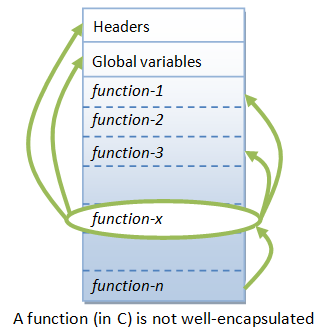
\includegraphics[scale=0.6]{OOP_CFunction.png}
\end{center}
\end{figure}
Object-oriented programming (OOP) languages are designed to overcome these problems.
\subsection*{Object-Oriented Programming (OOP)}
The basic unit of OOP is a \texttt{class}, which encapsulates both the static properties and dynamic operations within a ``box'', and specifies the public interface for using these boxes. Since classes are well-encapsulated, it is easier to reuse these classes. In other words, OOP combines the data structures and algorithms of a software entity inside the same box.

OOP languages permit higher level of abstraction for solving real-life problems. The traditional procedural language (such as C and Pascal) forces you to think in terms of the structure of the computer (e.g. memory bits and bytes, array, decision, loop) rather than thinking in terms of the problem you are trying to solve. The OOP languages (such as Java, C++ and C\#) let you think in the problem space, and use software objects to represent and abstract entities of the problem space to solve the problem.

\begin{figure}[H]
\begin{center}
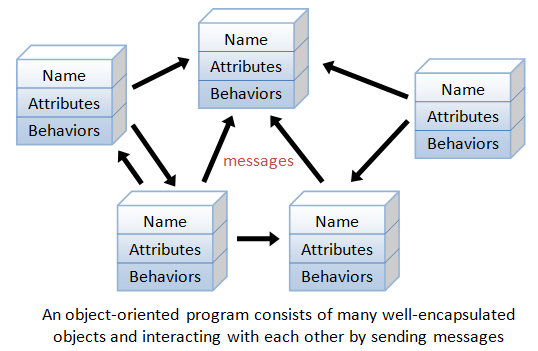
\includegraphics[scale=0.6]{OOP_Objects.png}
\end{center}
\end{figure}
As an example, suppose you wish to write a computer soccer game (considered as a complex application). It is quite difficult to model the game in procedural-oriented languages. But using OOP languages, you can easily model the program accordingly to the ``real things'' in the soccer game. For example Player entity can be elaborated as following.
\begin{itemize}
\item \texttt{Player:} attributes include name, number, location in the field, and etc; operations include run, jump, kick-the-ball, and etc.
\end{itemize}
\vfill{\ }
\begin{figure}[H]
\begin{center}
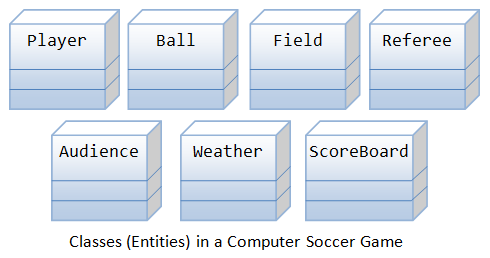
\includegraphics[scale=0.7]{OOP_SoccerGame.png}
\end{center}
\end{figure}

Similarly the other entities can have their own attributes and behaviour. Most importantly, some of these classes (such as Ball and Audience) can be reused in another application, e.g., computer basketball game, with little or no modification.

\section*{OOPs Concepts}
The basic OOPs concepts are:
\begin{enumerate}
\item Class
\item Objects
\item Abstraction
\item Encapsulation
\item Inheritance
\item Polymorphism
\end{enumerate}
\subsection*{Class}
In Java, a class is a definition of objects of the same kind. In other words, a class is a blueprint, template, or prototype that defines and describes the static attributes and dynamic behaviors common to all objects of the same kind.

An instance is a realization of a particular item of a class. In other words, an instance is an instantiation of a class. All the instances of a class have similar properties, as described in the class definition. For example, you can define a class called ``Student'' and create three instances of the class ``Student'' for ``Peter'', ``Paul'' and ``Pauline''.

The term ``object'' usually refers to instance. But it is often used loosely, which may refer to a class or an instance.

\subsubsection*{A Class is a 3-Compartment Box encapsulating Data and Operations}
A class can be visualized as a three-compartment box, as illustrated:

\fbox{
\begin{tabular}{l l}
\begin{minipage}{0.25\textwidth}
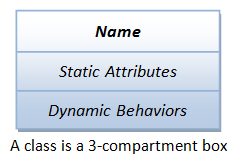
\includegraphics[scale=.8]{OOP_ThreeCompartment.png}
\end{minipage}
&
\begin{minipage}{0.65\textwidth}
\begin{enumerate}
\item \texttt{Name (or identity):} identifies the class.
\item \texttt{Variables (or attribute, state, field):} contains the static attributes of the class.
\item \texttt{Methods (or behaviors, function, operation):} contains the dynamic behaviors of the class.
\end{enumerate}
\end{minipage}
\end{tabular}
}

The following figure shows a few examples of classes and two instances of the class \texttt{Student}, identified as ``\texttt{paul}'' and ``\texttt{peter}''.

\begin{figure}[H]
\centering
\begin{minipage}[c]{0.5\linewidth}
\frame{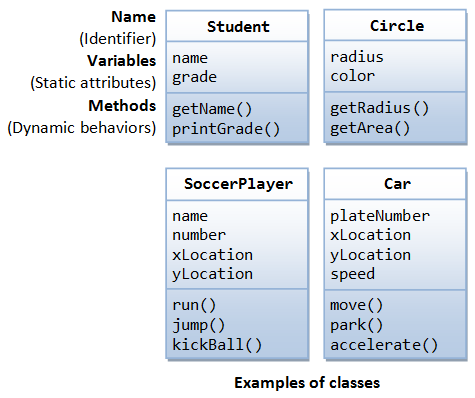
\includegraphics[scale=0.6]{OOP_ClassExamples.png}}
\end{minipage}
\quad
\begin{minipage}[c]{0.40\linewidth}
\frame{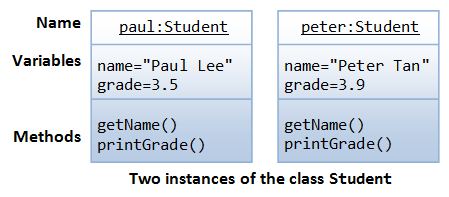
\includegraphics[width=5.5cm, height=4cm]{OOP_InstanceExamples.png}}
\end{minipage}
\end{figure}
\subsubsection*{Syntax:}
\begin{lstlisting}[numbers=none, xleftmargin=.25in]
[AccessControlModifier] class ClassName {
   // class body contains definition of variables and methods
   ...
}
\end{lstlisting}
\subsubsection*{Class Definition}
In Java, we use the keyword \texttt{class} to define a class. For examples:
\begin{lstlisting}[numbers=none, xleftmargin=.25in]
public class Circle { 
    // variables
    double radius;    
    String color;
    // methods
    double getRadius() {...}
    double getArea() {...}
}
\end{lstlisting} 

\subsection*{Objects}
A thing in a real world that can be either physical or conceptual. An object in object oriented programming can be physical or conceptual.

Conceptual objects are entities that are not tangible in the way real world physical objects are. Bulb is a physical object. While college is a conceptual object. Conceptual objects may not have a real world equivalent. For instance, a Stack object in a program.

Object has state and behavior.

To create an instance of a class, you have to:
\begin{enumerate}
\item Declare an instance identifier (instance name) of a particular class.
\item Construct the instance (i.e., allocate storage for the instance and initialize the instance) using the ``\texttt{new}'' operator.
\end{enumerate}
For example, suppose that we have a class called \texttt{Circle}, we can create instances of \texttt{Circle} as follows:
\begin{lstlisting}[numbers=none, xleftmargin=.25in]
// Declare 3 instances of the class Circle, c1, c2, and c3
Circle c1, c2, c3;
// Allocate and construct the instances via new operator
c1 = new Circle();
c2 = new Circle(2.0);
c3 = new Circle(3.0, "red");
// You can declare and construct in the same statement
Circle c4 = new Circle();
\end{lstlisting} 
\vfill{\ }
\begin{figure}[H]
 \begin{center}
   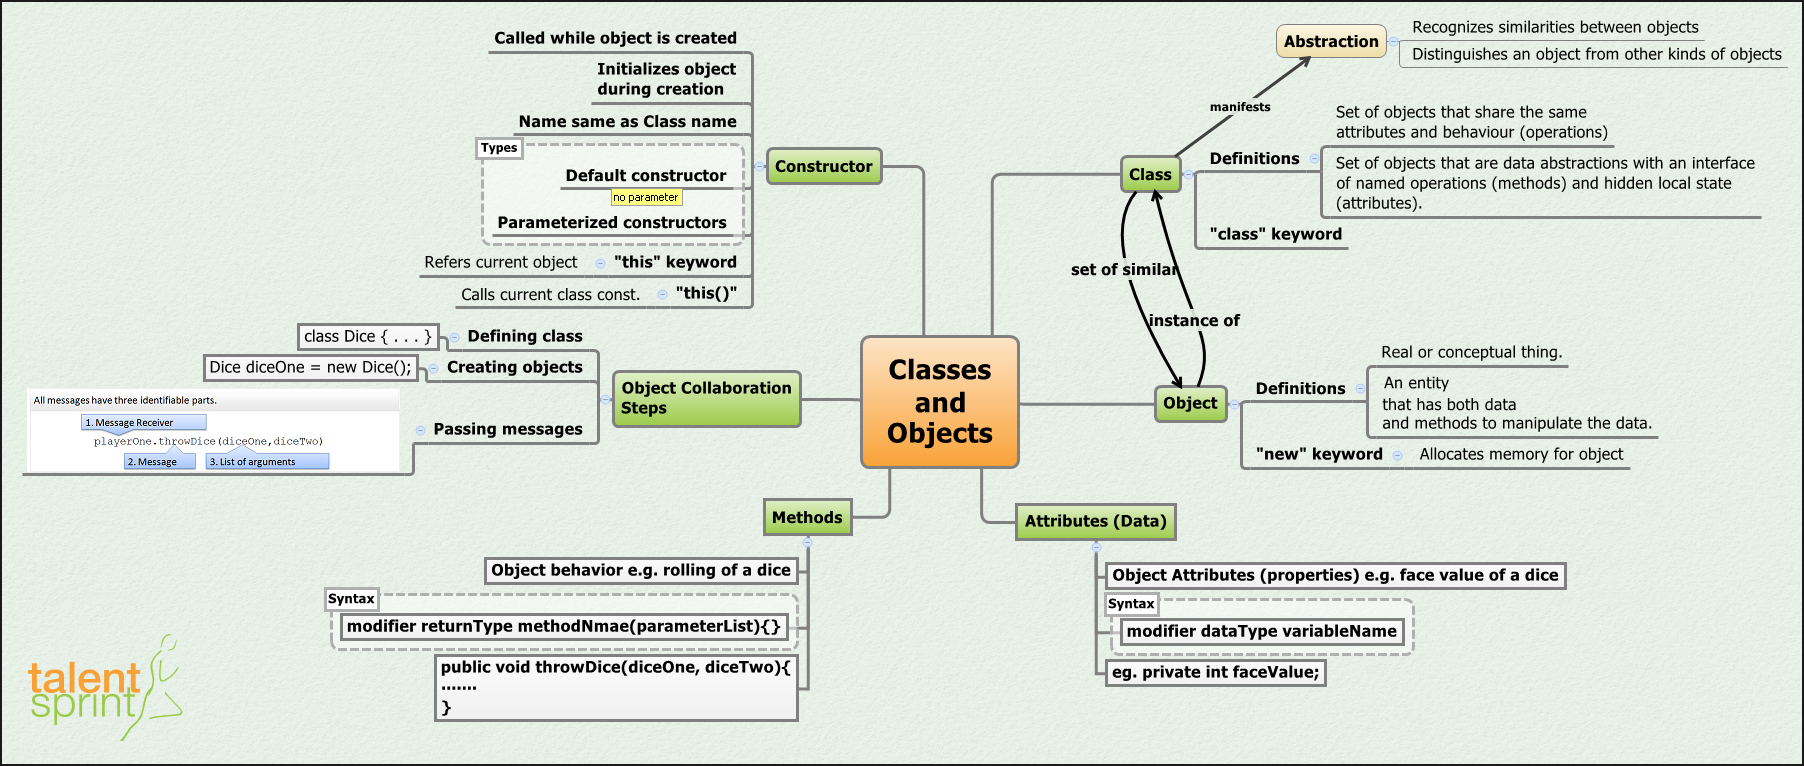
\includegraphics[angle=90,height=20cm, width=13cm]{ClassesAndObjects.png}
   
 \end{center}
 \end{figure}
\subsection*{Abstraction}
One of the chief advantages of object oriented programming is the idea that programmers can essentially focus on the ``big picture'' and ignore specific details regarding the inner-workings of an object. This concept is called abstraction.


For example a car in itself is a well-defined object, which is composed of several other smaller objects like a gearing system, steering mechanism, engine, which are again have their own subsystems. But for humans car is a one single object, which can be managed by the help of its subsystems, even if their inner details are unknown.

\subsection*{Encapsulation}
\begin{itemize}
\item Abstraction in OOP is closely related to a concept called encapsulation.
\item The Object Orientation has two major promises/benefits. They are: flexibility and maintainability.
\item You have to write your classes and code in a way that supports flexibility and maintainability.
\item The ability to make changes in your implementation code without breaking the code of others who use your code is a key benefit of encapsulation.
\item If you want maintainability, flexibility and extensibility your design must include encapsulation.
\item Encapsulation is the mechanism that binds together the code and the data it manipulates, and keeps both safe from outside interference and misuse.
\item The following are some of the ways to include encapsulation:
\begin{itemize}
\item Keep instance variables protected (with an access modifier, often private).
\item Make public accessor methods, and force calling code to use those methods rather than directly accessing the instance variable.
\item For the methods, use the JavaBeans naming convention or follow lowerCamelCase convention 
\begin{lstlisting}[numbers=none, xleftmargin=.15in]
set<someProperty> and get<someProperty> or isStudentApproved()
\end{lstlisting} 
\end{itemize}

\begin{figure}[H]
\begin{center}
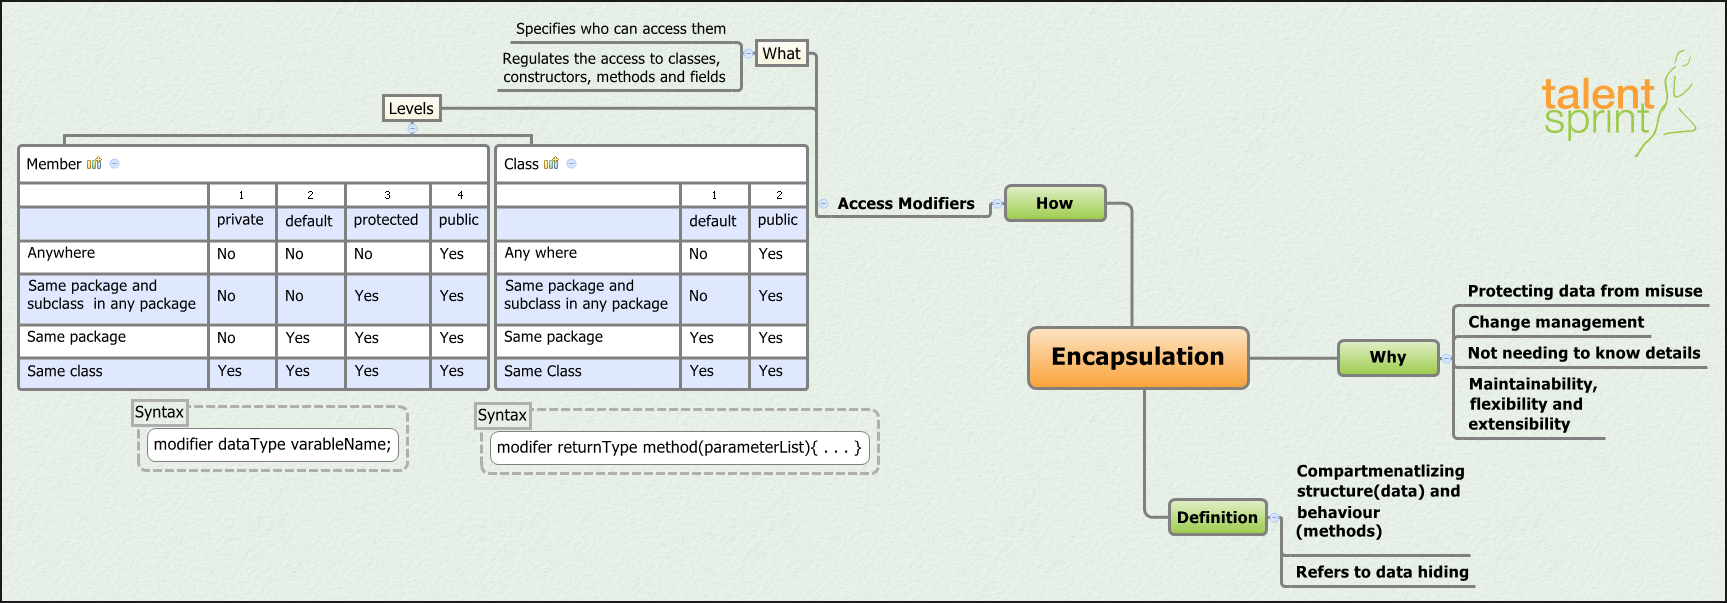
\includegraphics[angle=90,height=20cm, width=13cm]{EncapsulationMM.png}
\end{center}
\end{figure}

\end{itemize}
Looking at the example of a power steering mechanism of a car. Power steering of a car is a complex system, which internally have lots of components tightly coupled together, they work synchronously to turn the car in the desired direction. It even controls the power delivered by the engine to the steering wheel. But to the external world there is only one interface available and rest of the complexity is hidden. Moreover, the steering unit in itself is complete and independent. It does not affect the functioning of any other mechanism.
\subsection*{Inheritance}
One of the main concept of OOP is inheritance.

A child class inherits properties and attributes from its parents. 

Inheritance is the process by which one class acquires the properties of another class. By use of inheritance, a class needs only to define all of its characteristics that make it unique within its class; it can inherit its general attributes from its parent.

The derived class contains all the attributes and behaviors of its parent class. Moreover the derived class can define its own attributes and behaviors.

The derived class can override the definition of existing methods by providing its own implementation.

The code of the derived class consists only the changes and additions to the base class.

\subsubsection*{Need of Inheritance}
Inheritance is required for the following reasons:

Modular coding, which means less code and easier to get an idea about the code
\begin{itemize}
\item Code reuse
\item Do not break what is already working
\item Easier updates
\end{itemize}

For example, Car is a classification of Four Wheeler. Here Car acquires the properties of a four-wheeler. Other classifications could be a jeep, tempo, van etc. Four Wheeler defines a class of vehicles that have four wheels, and specific range of engine power, load carrying capacity etc. Car (termed as a sub-class) acquires these properties from Four Wheeler (termed as a super-class), and has some specific properties, which are different from other classifications of Four Wheeler, such as luxury, comfort, shape, size, usage etc.

A car can have further classification such as an open car, small car, big car etc, which will acquire the properties from both Four Wheeler and Car, but will still have some specific properties. This way the level of hierarchy can be extended to any level.

Java Swing and Awt classes represent best examples for inheritance.
\subsection*{Polymorphism}
Polymorphism (from Greek, meaning ``many forms'') is a feature that allows one interface to be used for a general class of actions that is one interface with multiple methods.

Generally, polymorphism allows you to mix methods and objects of different types in a consistent way.

Lets us look at same example of a car. A car have a gear transmission system. It has four front gears and one backward gear. When the engine is accelerated then depending upon which gear is engaged different amount power and movement is delivered to the car.

Polymorphism could be static and dynamic both. \textbf{Overloading} is static polymorphism, where, \textbf{overriding} is dynamic polymorphism.

\subsubsection*{Method Overloading}
In this case, different methods within the same class or in a common hierarchy share the same name but have different method signatures (name + parameters).
\begin{lstlisting}[numbers=none, xleftmargin=.25in]
public static float max(float a, float b)
public static float max(float a, float b, float c)
public static int max(int a, int b)
\end{lstlisting}
When a method is called, the call signature is matched to the correct method version.

\textbf{Note:} This is done during program compilation

\section*{Object class}
Every class in Java extends class \textbf{Object} which is stored in the \textbf{java.lang package} and is the ultimate superclass of all Java classes (except for Object).

Any class that does not explicitly extend another class, implicitly extends \texttt{Object} class.

Few important methods of the \texttt{Object} class are as follows:
\begin{description}
\item [equals(Object obj):]  Indicates whether some other object is ``equal to'' this one and it returns a boolean value as true or false
\item [toString():] Returns a string representation of the object
\item [hashCode():] Returns a hash code value (of integer type) for the object
\end{description}
\section*{Instance and Local Variables}
\subsection*{Instance (or member) Variables}
\begin{itemize}
\item Accessible anywhere in the class
\item Automatically initialized before invoking any constructor
\item Static variables are initialized at class load time
\item Can have the same name as the class
\item This differentiates one object from another, giving an object its individuality. For example, the particular \texttt{name} and address for a given \texttt{Person} object is declared as an instance variable.
\item An instance variable relates to an instance (object) of its class.

\end{itemize}
\begin{lstlisting}[numbers=none, xleftmargin=.25in]
class Person {
    private String name;
    public void setName(String aName) {
        name = aName;
    }
    public String getName() {
        return name;
    }
}
\end{lstlisting}
Here, instance variable called \texttt{name} of type \texttt{String} declared inside the class \texttt{Person}.
\subsection*{Local Variables}
\begin{itemize}
\item Must be initialized explicitly and (Or, the compiler will catch it.) Object references can be initialized to \texttt{null}.

\item The following code will not compile. Specify else part or initialize the local variable explicitly.
\begin{lstlisting}[numbers=none, xleftmargin=.25in]
public String testMethod(int a) {
    String tmp;
    if (a > 0)
        tmp = ``Positive'';
    return tmp;
}
\end{lstlisting}
Can have the same name as a member variable and resolution is based on scope.
\end{itemize}
 
 \end{document}
